\chapter{Wave Analysis}
\label{c:wave}

%----------------------------------------------------------------
\section{General Description}
\label{s:wave.general}

A ``wave analysis'' is method for finding isolated ``kick errors'' in a machine by analyzing the
appropriate data. Types of data that can be analyzed and the associated error type is shown in
Table~\ref{t:wave0}.

The analysis works on difference quantities. For example, the difference between measurement and
theory or the difference between two measurements, etc. Orbit and vertical dispersion measurements
are the exception here since an analysis of, say, just an orbit measurement can be considered to be
the difference between the measurement and a perfectly flat (zero) orbit.

\begin{table}[h]
\centering{\tt
\begin{tabular}{ll} \toprule
  {\it Measurement Type}     & {\it Error Type}           \\ \midrule
  Orbit                      & Steering errors            \\
  Betatron phase differences & Quadrupolar errors         \\
  Beta function differences  & Quadrupolar errors         \\
  Coupling                   & Skew quadrupolar errors    \\
  Dispersion differences     & Sextupole errors           \\ \bottomrule
\end{tabular}}
\caption[Wave measurement types.]
{Types of measurements that can be used in a wave analysis and the 
types of errors that can be diagnosed.}
\label{t:wave0}
\end{table}

\begin{figure}[t]
  \centering
  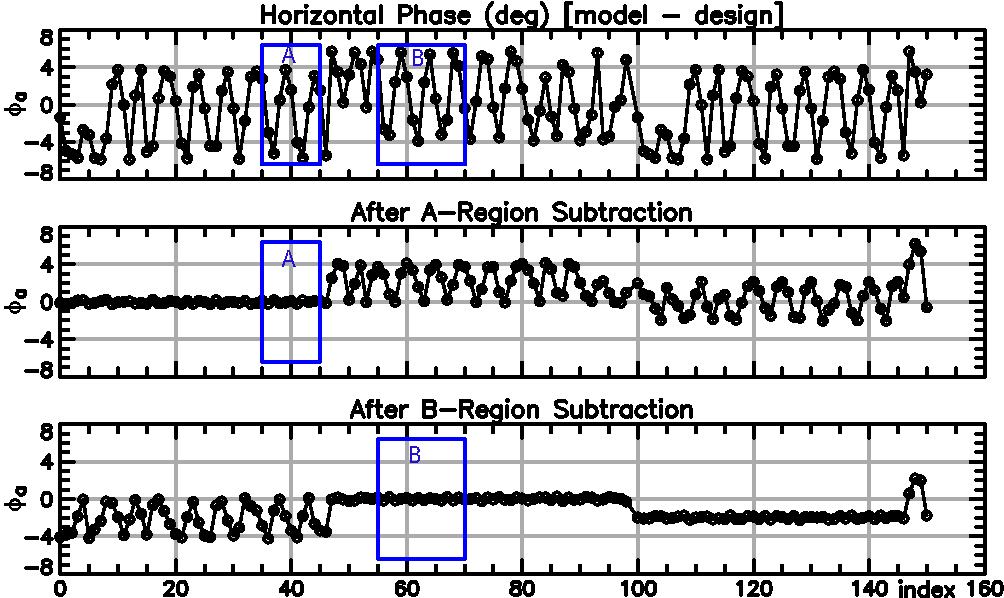
\includegraphics[width=6in]{wave.pdf}
  \caption[Example wave analysis.]
{Example wave analysis for betatron phase data.}
  \label{f:wave}
\end{figure}

The formulation of the wave analysis for quadrupolar and skew quadrupolar errors is presented by
Sagan\cite{b:wave}.  Although not discussed in the paper, the wave analysis for orbit and dispersion
measurements is similar to the beta function analysis that is presented.

The wave analysis is similar for all the measurement types. How the wave analysis works is
illustrated in Figure~\ref{f:wave}.  Figure~\ref{f:wave}a shows the difference between \vn{model}
and \vn{design} values for the $a$-mode betatron phase for the Cornell's Cesr storage ring. In this
example, one quadrupole in the model has been varied from it's design value. The horizontal axis is
the detector index.

For the wave analysis, two regions of the machine, labeled $A$ and $B$ in the figure, are chosen
(more on this later). For each region in turn, the data in that region is fit using a functional
form that assumes that there are no kick errors in the regions.  For phase differences, this
functional form is
\Begineq
  \delta \phi(s) = D \, \sin(2 \, \phi(s) + \phi_0) + C
  \label{xabps}
\Endeq
where $\phi$ is the phase advance and the quantities $C$, $D$ and $\phi_0$ are varied to give the
best fit.  Once $C$, $D$, and $\phi_0$ are fixed, \Eq{xabps} can be evaluated at any
point. Figure~\ref{f:wave}b shows the orbit of \ref{f:wave}a with the fit to the $A$ region
subtracted off. Similarly, Figure~\ref{f:wave}c shows the orbit of Figure~\ref{f:wave}a with the fit
to the $B$ region subtracted off. Concentrating on Figure~\ref{f:wave}b, since there are no kick
errors in the $A$ region, the fit is very good and hence the difference between the data and the fit
is nearly zero. Moving to the right from the $A$ region in Figure~\ref{f:wave}b, this difference is
nearly zero up to where the assumption of no kick errors is violated. That is, at the location of
the quadrupole error near detector 47. Similarly, since there are no kick errors in region $B$, the
difference between the data and the $B$ region fit is nearly zero in Figure~\ref{f:wave}c and this
remains true moving leftward from region $B$ up to the quadrupole near detector 47.

By taking the fitted values for $C$, $D$, and $\phi_0$ for the regions $A$ and $B$, the point
between the regions where the kick is generated and the amplitude of the kick can be
calculated. This calculation is similar to that used to find quadrupolar errors from beta
data\ref{f:wave}. The one difference is a factor of 2 that appears in the beta calculation due to
the fact that a freely propagating beta wave oscillates at $2\phi(s)$.

The success of the wave analysis in finding a kick error depends upon whether there are regions of
sufficient size on both sides of the kick that are kick error free. That is, whether the kick error
is ``isolated''. The locations of the $A$ and $B$ regions are set by the user and the general
strategy is to try to find, by varying the location of the regions, locations where the data is well
fit within the regions. The data is well fit if the difference between data and fit is small
compared to the data itself. If there are multiple isolated kick errors, then each error in turn can
be bracketed and analyzed. If there are multiple errors so close together that they cannot be
resolved, this will throw off the analysis, but it may still be possible to give bounds for the
location where the kicks are at and an ``effective'' kick amplitude can be calculated.

For circular machines, to be able to analyze kicks near the beginning or end of the lattice, the
wave analysis can be done by ``wrapping'' the data past the end of the lattice for another 1/2
turn. This is illustrated in Figure~\ref{f:wave}. In the Cesr machine, there are approximately 100
detectors labeled from 0 to 99.  The detectors from 100 to 150 are just the detectors from 0 to 50
shifted by 100. Thus, for example, the detector labeled 132 in the figure is actually detector 32.

%----------------------------------------------------------------
\section{Wave Analysis in Tao}
\label{s:wave.tao}

Performing a wave analysis in \tao is a three step process:
\begin{example}
  1) Plot the data to be analyzed.
  2) Use the \vn{wave} command to select the data.
  3) Use the \vn{set wave} command to vary the fit regions.
\end{example}

In general, the accuracy of the wave analysis depends upon the accuracy with which the beta function
and phase advances are known in the baseline lattice used. \tao uses the \vn{model} lattice for the
baseline. If possible, One strategy to improve the accuracy of the wave analysis is first use a
measurement to calculate what the quadrupole strengths in the \vn{model} lattice should be. Possible
measurements that can give this information include an orbit response matrix (ORM) analysis, fits to
beta or betatron phase measurements, etc.

%----------------------------------------------------------------
\section{Preparing the Data} 
\label{s:wave.data}

At present (due to limited manpower to do the coding), the wave analysis is restricted to data that
is stored in a \vn{d1_data} array (\sref{c:data}). That is, the plotted curve to be analyzed must
have its \vn{data_type} parameter set to \vn{``data''} (\sref{s:init.data}). The possible data types
that can be analyzed are:
\begin{example}
  orbit.x, orbit.y
  beta.a,  beta.b
  phase.a, phase.b
  eta.x, eta.y
  cbar.11, cbar.12, cbar.21      ! Analysis not possible for cbar.21
  ping_a.amp_x, ping_a.phase_x
  ping_a.sin_y, ping_a.cos_y
  ping_b.amp_y, ping_b.phase_y
  ping_b.sin_x, ping_b.cos_x
\end{example}
The curve to be analyzed must be visible. Any combination of data components may be used:. "meas",
"meas-ref", "model", etc.

If data from a circular machine is being analyzed, the data is wrapped past the end of the lattice
for another 1/2 turn. The translation from the data index in the wrapped section to the first 1/2
section of the lattice is determined by the values of \vn{ix_min_data} and \vn{ix_max_data} of the
\vn{d1_data} array under consideration (\sref{s:init.data}):
\begin{example}
  index_wrap \(\longrightarrow\) index_wrap - (ix_max_data - ix_min_data + 1)
\end{example}
For example, for the Cesr example in the previous section, \vn{ix_min_data} was 0 and
\vn{ix_max_data} was 99 to the translation was
\begin{example}
  index_wrap \(\longrightarrow\) index_wrap - 100
\end{example}

%----------------------------------------------------------------
\section{Wave Analysis Commands and Output}
\label{s:wave.cmd.out}

The \vn{wave} command (\sref{s:wave}) sets which plotted data curve is used for the wave
analysis. The \vn{set wave} command (\sref{s:set}) is used for setting the $A$ and $B$ region
locations. Finally the \vn{show wave} command (\sref{s:show}) prints analysis results.

Example wave analysis output with \vn{show wave}:
\begin{example}
  ix_a:  35  45
  ix_b:  55  70
  A Region Sigma_Fit/Amp_Fit:     0.018
  B Region Sigma_Fit/Amp_Fit:     0.015
  Sigma_Kick/Kick:    0.013
  Sigma_phi:          0.019
  Chi_C:              0.037 [Figure of Merit]

  Normalized Kick = k * l * beta [dimensionless]
     where k = quadrupole gradient [rad/m^2].
  After Dat#     Norm_K       phi
         46      0.0705    30.431
         49      0.0705    33.573
         53      0.0705    36.715
\end{example}
This output is for analysis of betatron phase data but the output for other types of data is
similar.  The first two lines of the output show where the $A$ and $B$ regions are. The next two
lines show $\sigma_{a}/A_a$ and $\sigma_{b}/A_b$ where $\sigma_a$ and $\sigma_b$ are given by
Eq.~(42) of Sagan\cite{b:wave} and
\Begineq
  A_a \equiv \sqrt{\xi_a^2 + \eta_a^2}
\Endeq
with a similar equation for $A_b$. $\sigma_{a}/A_a$ and $\sigma_{b}/A_b$ are thus a measure of how
well the data is fit in the $A$ and $B$ regions with a value of zero being a perfect fit and a value
of one indicating a poor fit. Notice that a poor fit of one of the regions may simply be a
reflection that the wave amplitude being there. The next three lines of the output are
$\sigma_{\delta k}/\delta k$, $\sigma_\phi$, and $\xi_C$, and are given by Eq.~(39), (43), and (44)
respectively of \cite{b:wave}. The last three lines of the analysis tell where the wave analysis
predicts the kicks are and what the normalized kick amplitudes are. Thus the first of these three
lines indicates that the kick may be somewhere after the location of datum \#46 (but before the
location of datum \#47), The normalized quadrupole kick amplitude is 0.0705, and the betatron phase
at the putative kick is 30.431 radians.
